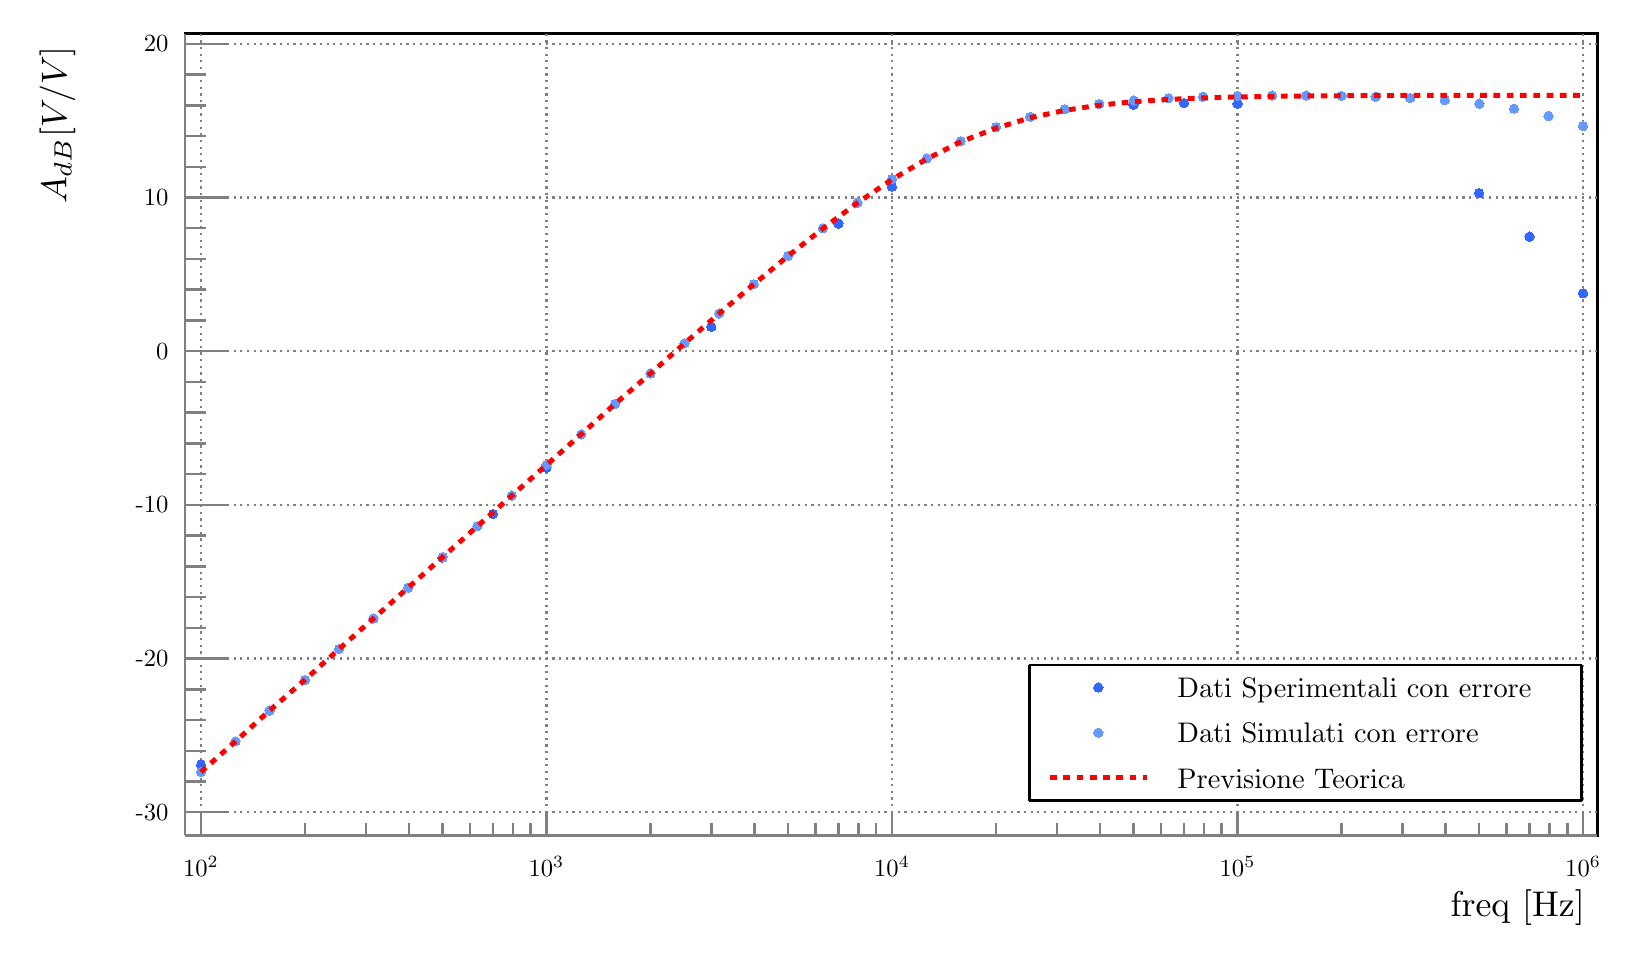
\begin{tikzpicture}
\pgfdeclareplotmark{cross} {
\pgfpathmoveto{\pgfpoint{-0.3\pgfplotmarksize}{\pgfplotmarksize}}
\pgfpathlineto{\pgfpoint{+0.3\pgfplotmarksize}{\pgfplotmarksize}}
\pgfpathlineto{\pgfpoint{+0.3\pgfplotmarksize}{0.3\pgfplotmarksize}}
\pgfpathlineto{\pgfpoint{+1\pgfplotmarksize}{0.3\pgfplotmarksize}}
\pgfpathlineto{\pgfpoint{+1\pgfplotmarksize}{-0.3\pgfplotmarksize}}
\pgfpathlineto{\pgfpoint{+0.3\pgfplotmarksize}{-0.3\pgfplotmarksize}}
\pgfpathlineto{\pgfpoint{+0.3\pgfplotmarksize}{-1.\pgfplotmarksize}}
\pgfpathlineto{\pgfpoint{-0.3\pgfplotmarksize}{-1.\pgfplotmarksize}}
\pgfpathlineto{\pgfpoint{-0.3\pgfplotmarksize}{-0.3\pgfplotmarksize}}
\pgfpathlineto{\pgfpoint{-1.\pgfplotmarksize}{-0.3\pgfplotmarksize}}
\pgfpathlineto{\pgfpoint{-1.\pgfplotmarksize}{0.3\pgfplotmarksize}}
\pgfpathlineto{\pgfpoint{-0.3\pgfplotmarksize}{0.3\pgfplotmarksize}}
\pgfpathclose
\pgfusepathqstroke
}
\pgfdeclareplotmark{cross*} {
\pgfpathmoveto{\pgfpoint{-0.3\pgfplotmarksize}{\pgfplotmarksize}}
\pgfpathlineto{\pgfpoint{+0.3\pgfplotmarksize}{\pgfplotmarksize}}
\pgfpathlineto{\pgfpoint{+0.3\pgfplotmarksize}{0.3\pgfplotmarksize}}
\pgfpathlineto{\pgfpoint{+1\pgfplotmarksize}{0.3\pgfplotmarksize}}
\pgfpathlineto{\pgfpoint{+1\pgfplotmarksize}{-0.3\pgfplotmarksize}}
\pgfpathlineto{\pgfpoint{+0.3\pgfplotmarksize}{-0.3\pgfplotmarksize}}
\pgfpathlineto{\pgfpoint{+0.3\pgfplotmarksize}{-1.\pgfplotmarksize}}
\pgfpathlineto{\pgfpoint{-0.3\pgfplotmarksize}{-1.\pgfplotmarksize}}
\pgfpathlineto{\pgfpoint{-0.3\pgfplotmarksize}{-0.3\pgfplotmarksize}}
\pgfpathlineto{\pgfpoint{-1.\pgfplotmarksize}{-0.3\pgfplotmarksize}}
\pgfpathlineto{\pgfpoint{-1.\pgfplotmarksize}{0.3\pgfplotmarksize}}
\pgfpathlineto{\pgfpoint{-0.3\pgfplotmarksize}{0.3\pgfplotmarksize}}
\pgfpathclose
\pgfusepathqfillstroke
}
\pgfdeclareplotmark{newstar} {
\pgfpathmoveto{\pgfqpoint{0pt}{\pgfplotmarksize}}
\pgfpathlineto{\pgfqpointpolar{44}{0.5\pgfplotmarksize}}
\pgfpathlineto{\pgfqpointpolar{18}{\pgfplotmarksize}}
\pgfpathlineto{\pgfqpointpolar{-20}{0.5\pgfplotmarksize}}
\pgfpathlineto{\pgfqpointpolar{-54}{\pgfplotmarksize}}
\pgfpathlineto{\pgfqpointpolar{-90}{0.5\pgfplotmarksize}}
\pgfpathlineto{\pgfqpointpolar{234}{\pgfplotmarksize}}
\pgfpathlineto{\pgfqpointpolar{198}{0.5\pgfplotmarksize}}
\pgfpathlineto{\pgfqpointpolar{162}{\pgfplotmarksize}}
\pgfpathlineto{\pgfqpointpolar{134}{0.5\pgfplotmarksize}}
\pgfpathclose
\pgfusepathqstroke
}
\pgfdeclareplotmark{newstar*} {
\pgfpathmoveto{\pgfqpoint{0pt}{\pgfplotmarksize}}
\pgfpathlineto{\pgfqpointpolar{44}{0.5\pgfplotmarksize}}
\pgfpathlineto{\pgfqpointpolar{18}{\pgfplotmarksize}}
\pgfpathlineto{\pgfqpointpolar{-20}{0.5\pgfplotmarksize}}
\pgfpathlineto{\pgfqpointpolar{-54}{\pgfplotmarksize}}
\pgfpathlineto{\pgfqpointpolar{-90}{0.5\pgfplotmarksize}}
\pgfpathlineto{\pgfqpointpolar{234}{\pgfplotmarksize}}
\pgfpathlineto{\pgfqpointpolar{198}{0.5\pgfplotmarksize}}
\pgfpathlineto{\pgfqpointpolar{162}{\pgfplotmarksize}}
\pgfpathlineto{\pgfqpointpolar{134}{0.5\pgfplotmarksize}}
\pgfpathclose
\pgfusepathqfillstroke
}
\definecolor{c}{rgb}{1,1,1};
\draw [color=c, fill=c] (0,0) rectangle (20,11.523);
\draw [color=c, fill=c] (1.98397,1.30261) rectangle (19.9198,11.483);
\definecolor{c}{rgb}{0,0,0};
\draw [c,line width=0.9] (1.98397,1.30261) -- (1.98397,11.483) -- (19.9198,11.483) -- (19.9198,1.30261) -- (1.98397,1.30261);
\definecolor{c}{rgb}{1,1,1};
\draw [color=c, fill=c] (1.98397,1.30261) rectangle (19.9198,11.483);
\definecolor{c}{rgb}{0,0,0};
\draw [c,line width=0.9] (1.98397,1.30261) -- (1.98397,11.483) -- (19.9198,11.483) -- (19.9198,1.30261) -- (1.98397,1.30261);
\definecolor{c}{rgb}{0.5,0.5,0.5};
\draw [c,line width=0.9] (1.98397,1.30261) -- (19.9198,1.30261);
\draw [c,dash pattern=on 0.80pt off 1.60pt ,line width=0.9] (2.18476,11.483) -- (2.18476,1.30261);
\draw [c,dash pattern=on 0.80pt off 1.60pt ,line width=0.9] (6.57313,11.483) -- (6.57313,1.30261);
\draw [c,dash pattern=on 0.80pt off 1.60pt ,line width=0.9] (10.9615,11.483) -- (10.9615,1.30261);
\draw [c,dash pattern=on 0.80pt off 1.60pt ,line width=0.9] (15.3498,11.483) -- (15.3498,1.30261);
\draw [c,dash pattern=on 0.80pt off 1.60pt ,line width=0.9] (19.7382,11.483) -- (19.7382,1.30261);
\draw [c,line width=0.9] (1.98397,1.30261) -- (1.98397,11.483);
\draw [c,dash pattern=on 0.80pt off 1.60pt ,line width=0.9] (19.9198,1.59513) -- (1.98397,1.59513);
\draw [c,dash pattern=on 0.80pt off 1.60pt ,line width=0.9] (19.9198,3.54688) -- (1.98397,3.54688);
\draw [c,dash pattern=on 0.80pt off 1.60pt ,line width=0.9] (19.9198,5.49864) -- (1.98397,5.49864);
\draw [c,dash pattern=on 0.80pt off 1.60pt ,line width=0.9] (19.9198,7.4504) -- (1.98397,7.4504);
\draw [c,dash pattern=on 0.80pt off 1.60pt ,line width=0.9] (19.9198,9.40215) -- (1.98397,9.40215);
\draw [c,dash pattern=on 0.80pt off 1.60pt ,line width=0.9] (19.9198,11.3539) -- (1.98397,11.3539);
\draw [c,dash pattern=on 0.80pt off 1.60pt ,line width=0.9] (19.9198,1.59513) -- (1.98397,1.59513);
\draw [c,dash pattern=on 0.80pt off 1.60pt ,line width=0.9] (19.9198,11.3539) -- (1.98397,11.3539);
\draw [c,line width=0.9] (1.98397,1.30261) -- (19.9198,1.30261);
\draw [c,line width=0.9] (2.18476,1.61262) -- (2.18476,1.30261);
\definecolor{c}{rgb}{0,0,0};
\draw [anchor=base] (2.18476,0.781188) node[scale=0.890168, color=c, rotate=0]{$10^{2}$};
\definecolor{c}{rgb}{0.5,0.5,0.5};
\draw [c,line width=0.9] (3.50579,1.45761) -- (3.50579,1.30261);
\draw [c,line width=0.9] (4.27854,1.45761) -- (4.27854,1.30261);
\draw [c,line width=0.9] (4.82682,1.45761) -- (4.82682,1.30261);
\draw [c,line width=0.9] (5.2521,1.45761) -- (5.2521,1.30261);
\draw [c,line width=0.9] (5.59957,1.45761) -- (5.59957,1.30261);
\draw [c,line width=0.9] (5.89336,1.45761) -- (5.89336,1.30261);
\draw [c,line width=0.9] (6.14785,1.45761) -- (6.14785,1.30261);
\draw [c,line width=0.9] (6.37233,1.45761) -- (6.37233,1.30261);
\draw [c,line width=0.9] (6.57313,1.61262) -- (6.57313,1.30261);
\definecolor{c}{rgb}{0,0,0};
\draw [anchor=base] (6.57313,0.781188) node[scale=0.890168, color=c, rotate=0]{$10^{3}$};
\definecolor{c}{rgb}{0.5,0.5,0.5};
\draw [c,line width=0.9] (7.89415,1.45761) -- (7.89415,1.30261);
\draw [c,line width=0.9] (8.66691,1.45761) -- (8.66691,1.30261);
\draw [c,line width=0.9] (9.21518,1.45761) -- (9.21518,1.30261);
\draw [c,line width=0.9] (9.64046,1.45761) -- (9.64046,1.30261);
\draw [c,line width=0.9] (9.98794,1.45761) -- (9.98794,1.30261);
\draw [c,line width=0.9] (10.2817,1.45761) -- (10.2817,1.30261);
\draw [c,line width=0.9] (10.5362,1.45761) -- (10.5362,1.30261);
\draw [c,line width=0.9] (10.7607,1.45761) -- (10.7607,1.30261);
\draw [c,line width=0.9] (10.9615,1.61262) -- (10.9615,1.30261);
\definecolor{c}{rgb}{0,0,0};
\draw [anchor=base] (10.9615,0.781188) node[scale=0.890168, color=c, rotate=0]{$10^{4}$};
\definecolor{c}{rgb}{0.5,0.5,0.5};
\draw [c,line width=0.9] (12.2825,1.45761) -- (12.2825,1.30261);
\draw [c,line width=0.9] (13.0553,1.45761) -- (13.0553,1.30261);
\draw [c,line width=0.9] (13.6035,1.45761) -- (13.6035,1.30261);
\draw [c,line width=0.9] (14.0288,1.45761) -- (14.0288,1.30261);
\draw [c,line width=0.9] (14.3763,1.45761) -- (14.3763,1.30261);
\draw [c,line width=0.9] (14.6701,1.45761) -- (14.6701,1.30261);
\draw [c,line width=0.9] (14.9246,1.45761) -- (14.9246,1.30261);
\draw [c,line width=0.9] (15.149,1.45761) -- (15.149,1.30261);
\draw [c,line width=0.9] (15.3498,1.61262) -- (15.3498,1.30261);
\definecolor{c}{rgb}{0,0,0};
\draw [anchor=base] (15.3498,0.781188) node[scale=0.890168, color=c, rotate=0]{$10^{5}$};
\definecolor{c}{rgb}{0.5,0.5,0.5};
\draw [c,line width=0.9] (16.6709,1.45761) -- (16.6709,1.30261);
\draw [c,line width=0.9] (17.4436,1.45761) -- (17.4436,1.30261);
\draw [c,line width=0.9] (17.9919,1.45761) -- (17.9919,1.30261);
\draw [c,line width=0.9] (18.4172,1.45761) -- (18.4172,1.30261);
\draw [c,line width=0.9] (18.7647,1.45761) -- (18.7647,1.30261);
\draw [c,line width=0.9] (19.0584,1.45761) -- (19.0584,1.30261);
\draw [c,line width=0.9] (19.3129,1.45761) -- (19.3129,1.30261);
\draw [c,line width=0.9] (19.5374,1.45761) -- (19.5374,1.30261);
\draw [c,line width=0.9] (19.7382,1.61262) -- (19.7382,1.30261);
\definecolor{c}{rgb}{0,0,0};
\draw [anchor=base] (19.7382,0.781188) node[scale=0.890168, color=c, rotate=0]{$10^{6}$};
\draw [anchor= east] (19.9198,0.380762) node[scale=1.29074, color=c, rotate=0]{freq [Hz]};
\definecolor{c}{rgb}{0.5,0.5,0.5};
\draw [c,line width=0.9] (1.98397,1.30261) -- (1.98397,11.483);
\draw [c,line width=0.9] (2.51405,1.59513) -- (1.98397,1.59513);
\draw [c,line width=0.9] (2.24901,1.98548) -- (1.98397,1.98548);
\draw [c,line width=0.9] (2.24901,2.37583) -- (1.98397,2.37583);
\draw [c,line width=0.9] (2.24901,2.76618) -- (1.98397,2.76618);
\draw [c,line width=0.9] (2.24901,3.15653) -- (1.98397,3.15653);
\draw [c,line width=0.9] (2.51405,3.54688) -- (1.98397,3.54688);
\draw [c,line width=0.9] (2.24901,3.93723) -- (1.98397,3.93723);
\draw [c,line width=0.9] (2.24901,4.32759) -- (1.98397,4.32759);
\draw [c,line width=0.9] (2.24901,4.71794) -- (1.98397,4.71794);
\draw [c,line width=0.9] (2.24901,5.10829) -- (1.98397,5.10829);
\draw [c,line width=0.9] (2.51405,5.49864) -- (1.98397,5.49864);
\draw [c,line width=0.9] (2.24901,5.88899) -- (1.98397,5.88899);
\draw [c,line width=0.9] (2.24901,6.27934) -- (1.98397,6.27934);
\draw [c,line width=0.9] (2.24901,6.66969) -- (1.98397,6.66969);
\draw [c,line width=0.9] (2.24901,7.06005) -- (1.98397,7.06005);
\draw [c,line width=0.9] (2.51405,7.4504) -- (1.98397,7.4504);
\draw [c,line width=0.9] (2.24901,7.84075) -- (1.98397,7.84075);
\draw [c,line width=0.9] (2.24901,8.2311) -- (1.98397,8.2311);
\draw [c,line width=0.9] (2.24901,8.62145) -- (1.98397,8.62145);
\draw [c,line width=0.9] (2.24901,9.0118) -- (1.98397,9.0118);
\draw [c,line width=0.9] (2.51405,9.40215) -- (1.98397,9.40215);
\draw [c,line width=0.9] (2.24901,9.79251) -- (1.98397,9.79251);
\draw [c,line width=0.9] (2.24901,10.1829) -- (1.98397,10.1829);
\draw [c,line width=0.9] (2.24901,10.5732) -- (1.98397,10.5732);
\draw [c,line width=0.9] (2.24901,10.9636) -- (1.98397,10.9636);
\draw [c,line width=0.9] (2.51405,11.3539) -- (1.98397,11.3539);
\draw [c,line width=0.9] (2.51405,1.59513) -- (1.98397,1.59513);
\draw [c,line width=0.9] (2.51405,11.3539) -- (1.98397,11.3539);
\definecolor{c}{rgb}{0,0,0};
\draw [anchor= east] (1.88397,1.59513) node[scale=0.890168, color=c, rotate=0]{-30};
\draw [anchor= east] (1.88397,3.54688) node[scale=0.890168, color=c, rotate=0]{-20};
\draw [anchor= east] (1.88397,5.49864) node[scale=0.890168, color=c, rotate=0]{-10};
\draw [anchor= east] (1.88397,7.4504) node[scale=0.890168, color=c, rotate=0]{0};
\draw [anchor= east] (1.88397,9.40215) node[scale=0.890168, color=c, rotate=0]{10};
\draw [anchor= east] (1.88397,11.3539) node[scale=0.890168, color=c, rotate=0]{20};
\draw [anchor= east] (0.362725,11.483) node[scale=1.29074, color=c, rotate=90]{$A_{dB} [V/V]$};
\definecolor{c}{rgb}{0.2,0.4,1};
\foreach \P in {(2.18477,2.19628), (5.2521,4.82963), (5.89336,5.38131), (6.57313,5.97179), (8.66691,7.75891), (10.2817,9.07078), (10.9615,9.53865), (14.0288,10.5789), (14.6701,10.6003), (15.3499,10.5923), (18.4172,9.45693), (19.0584,8.90525),
 (19.7382,8.18496)}{\draw[mark options={color=c,fill=c},mark size=1.681682pt, line width=0.000000pt, mark=*] plot coordinates {\P};}
\draw [c,line width=0.9] (2.18477,2.23636) -- (2.18477,2.24159);
\draw [c,line width=0.9] (2.14469,2.24159) -- (2.22485,2.24159);
\draw [c,line width=0.9] (2.18477,2.1562) -- (2.18477,2.15097);
\draw [c,line width=0.9] (2.14469,2.15097) -- (2.22485,2.15097);
\definecolor{c}{rgb}{0.4,0.6,1};
\foreach \P in {(2.18477,2.10524), (2.62523,2.49557), (3.05655,2.88589), (3.5058,3.27619), (3.93868,3.66647), (4.37758,4.0567), (4.81727,4.44686), (5.25591,4.83691), (5.69559,5.22678), (6.13351,5.61637), (6.57313,6.00552), (7.01359,6.39396),
 (7.44491,6.7813), (7.89416,7.1669), (8.32704,7.54978), (8.76594,7.92842), (9.20563,8.30053), (9.64427,8.66276), (10.0839,9.01036), (10.5219,9.33708), (10.9615,9.63545), (11.402,9.89782), (11.8333,10.1181), (12.2825,10.2939), (12.7154,10.427),
 (13.1543,10.5231), (13.594,10.5897), (14.0326,10.6343), (14.4723,10.6633), (14.9102,10.6814), (15.3499,10.6919), (15.7903,10.6967), (16.2216,10.6969), (16.6709,10.6925), (17.1038,10.6826), (17.5427,10.6653), (17.9824,10.6375), (18.421,10.5945),
 (18.8607,10.5302), (19.2986,10.4371), (19.7382,10.3077)}{\draw[mark options={color=c,fill=c},mark size=1.681682pt, line width=0.000000pt, mark=*] plot coordinates {\P};}
\definecolor{c}{rgb}{1,0,0};
\draw [c,dash pattern=on 2.40pt off 2.40pt ,line width=1.8] (2.18477,2.10524) -- (2.62523,2.49557) -- (3.05655,2.88589) -- (3.5058,3.27619) -- (3.93868,3.66647) -- (4.37758,4.05669) -- (4.81727,4.44685) -- (5.25591,4.83689) -- (5.69559,5.22675) --
 (6.13351,5.61633) -- (6.57313,6.00545) -- (7.01359,6.39385) -- (7.44491,6.78112) -- (7.89416,7.16662) -- (8.32704,7.54934) -- (8.76594,7.92772) -- (9.20563,8.29945) -- (9.64427,8.6611) -- (10.0839,9.00786) -- (10.5219,9.33342) -- (10.9615,9.63026)
 -- (11.402,9.89076) -- (11.8333,10.109) -- (12.2825,10.2827) -- (12.7154,10.414) -- (13.1543,10.5087) -- (13.594,10.5744) -- (14.0326,10.6187) -- (14.4723,10.6478) -- (14.9102,10.6667) -- (15.3499,10.6789) -- (15.7903,10.6867) -- (16.2216,10.6916)
 -- (16.6709,10.6947) -- (17.1038,10.6967) -- (17.5427,10.698) -- (17.9824,10.6988) -- (18.421,10.6993) -- (18.8607,10.6996) -- (19.2986,10.6998) -- (19.7382,10.6999);
\definecolor{c}{rgb}{1,1,1};
\draw [color=c, fill=c] (12.7054,1.74349) rectangle (19.7194,3.46693);
\definecolor{c}{rgb}{0,0,0};
\draw [c,line width=0.9] (12.7054,1.74349) -- (19.7194,1.74349);
\draw [c,line width=0.9] (19.7194,1.74349) -- (19.7194,3.46693);
\draw [c,line width=0.9] (19.7194,3.46693) -- (12.7054,3.46693);
\draw [c,line width=0.9] (12.7054,3.46693) -- (12.7054,1.74349);
\draw [anchor=base west] (14.4589,3.05043) node[scale=1.02369, color=c, rotate=0]{Dati Sperimentali con errore};
\definecolor{c}{rgb}{0.2,0.4,1};
\foreach \P in {(13.5822,3.17969)}{\draw[mark options={color=c,fill=c},mark size=1.681682pt, line width=0.000000pt, mark=*] plot coordinates {\P};}
\definecolor{c}{rgb}{0,0,0};
\draw [anchor=base west] (14.4589,2.47595) node[scale=1.02369, color=c, rotate=0]{Dati Simulati con errore};
\definecolor{c}{rgb}{0.4,0.6,1};
\foreach \P in {(13.5822,2.60521)}{\draw[mark options={color=c,fill=c},mark size=1.681682pt, line width=0.000000pt, mark=*] plot coordinates {\P};}
\definecolor{c}{rgb}{0,0,0};
\draw [anchor=base west] (14.4589,1.90147) node[scale=1.02369, color=c, rotate=0]{Previsione Teorica };
\definecolor{c}{rgb}{1,0,0};
\draw [c,dash pattern=on 2.40pt off 2.40pt ,line width=1.8] (12.9684,2.03073) -- (14.1959,2.03073);
\end{tikzpicture}
